\documentclass[../../main.tex]{subfiles}

\graphicspath{{../../image/}{../../figure/}}

\begin{document}

\section{权重衰减}\label{section:ch09-权重衰减}

我们在线性回归的背景下引入了正则化（参见\cref{subsection:ch01-正则化}）来控制模型的复杂性。这是一种限制模型中参数数量的替代方法。最简单的正则化项由模型参数的平方和构成，从而形成\eqref{align:ch09-正则化误差}的正则化误差函数。该误差函数会对较大的参数值施加惩罚。有效的模型复杂性由正则化系数 $\lambda$ 的选择决定。

我们还看到，这种加性的正则化项可以解释为权重向量 $\boldsymbol{w}$ 上零均值 Gauss 先验分布的负对数（参见\cref{section:ch02-Gauss分布}）。这为将先验知识纳入模型训练过程提供了概率性的视角。遗憾的是，这种先验是通过模型参数表示的，而我们具有的关于待解决问题的领域知识更可能是通过从输入到输出的网络函数形式表示的。然而，参数与网络函数之间的关系极其复杂，因此只有非常有限类型的先验知识可以直接轻松地表示为模型参数的先验。

\begin{proposition}[权重衰减的 Gauss 先验解释]\label{proposition:ch09-Gauss先验}
设 $\boldsymbol{w}\in\mathbb{R}^{M}$ 的先验分布为零均值各向同性 Gauss 分布 $p(\boldsymbol{w})=\mathcal{N}(\boldsymbol{w}\mid\boldsymbol{0},\alpha^{-1}\boldsymbol{I})$，其中 $\alpha>0$ 为精度。则负对数先验（忽略与 $\boldsymbol{w}$ 无关的常数）为
\begin{align*}
-\ln p(\boldsymbol{w})=\frac{\alpha}{2}\|\boldsymbol{w}\|^{2}+\text{常数}.
\end{align*}
因此，最小化\eqref{align:ch09-正则化误差}等价于在平方和误差下求最大后验（MAP）解，且 $\lambda=\alpha$。
\end{proposition}

\begin{proof}
（重构新增）由多元 Gauss 密度的定义，
\begin{align*}
p(\boldsymbol{w})=(2\pi)^{-M/2}\alpha^{M/2}\exp\!\left(-\frac{\alpha}{2}\boldsymbol{w}^{\mathsf T}\boldsymbol{w}\right),
\end{align*}
取负对数得
\begin{align*}
-\ln p(\boldsymbol{w})=\frac{\alpha}{2}\boldsymbol{w}^{\mathsf T}\boldsymbol{w}-\frac{M}{2}\ln\alpha+\frac{M}{2}\ln(2\pi).
\end{align*}
后两项与 $\boldsymbol{w}$ 无关，记为常数。于是
\begin{align*}
-\ln p(\boldsymbol{w}\mid\mathcal{D})=-\ln p(\mathcal{D}\mid\boldsymbol{w})-\ln p(\boldsymbol{w})+\text{常数}=E(\boldsymbol{w})+\frac{\alpha}{2}\|\boldsymbol{w}\|^{2}+\text{常数},
\end{align*}
其中 $E(\boldsymbol{w})=-\ln p(\mathcal{D}\mid\boldsymbol{w})$ 是负对数似然（对平方和误差即为其一半）。比较\eqref{align:ch09-正则化误差}即知 MAP 解与 $\lambda=\alpha$ 的正则化最小化解相同。
\end{proof}

% SUPPLEMENT: parent=proposition:ch09-Gauss先验; kind=motivation; location=紧随其后的 remark（重构新增）
\begin{remark}（重构新增）\cref{proposition:ch09-Gauss先验}说明二次惩罚不是随意的技巧，而是“参数先验为 Gauss 分布”这一假设的推论。精度 $\alpha$ 与正则化系数 $\lambda$ 一一对应：$\alpha$ 大（先验窄）等价于 $\lambda$ 大（强惩罚）。这也暴露了该先验的局限：它假设各参数独立、同方差、均值为零，而多层网络中不同层的权重尺度往往不同，因此实际使用分组或逐层的正则化系数（见\cref{definition:ch09-分组权重衰减}）。此外，把先验放在参数上而非函数上，是 Bayes 神经网络的主要困难：参数的对称性与缩放不变性会使先验在参数空间中“看起来”很窄，但在函数空间中未必如此。
\end{remark}

\eqref{align:ch09-正则化误差}中的平方和正则化项在机器学习文献中称为\textbf{权重衰减}（weight decay），因为在序贯学习算法中，它鼓励权重值向零衰减（除非数据支持其不衰减）（参见\cref{exercise:ch09-03}）。这种正则化项的一个优点是，它的导数很容易计算，可用于梯度下降训练。具体来说，对于\eqref{align:ch09-正则化误差}，梯度由下式给出：
\begin{align}
\nabla\widetilde{E}(\boldsymbol{w})=\nabla E(\boldsymbol{w})+\lambda\boldsymbol{w}.
\label{align:ch09-权重衰减梯度}
\end{align}
可以看到，\eqref{align:ch09-正则化误差}中的因子 $1/2$ 在取导数时会消失。

\begin{definition}[权重衰减]\label{definition:ch09-权重衰减}
称\eqref{align:ch09-正则化误差}中的二次正则化项 $\frac{\lambda}{2}\|\boldsymbol{w}\|^{2}$ 为\textbf{权重衰减}（weight decay），称相应的正则化训练为\textbf{权重衰减正则化}。其梯度由\eqref{align:ch09-权重衰减梯度}给出，即在原梯度上叠加 $\lambda\boldsymbol{w}$；在梯度下降更新中它表现为与参数成正比的回复项 $-\eta\lambda\boldsymbol{w}$。
\end{definition}

% SUPPLEMENT: parent=definition:ch09-权重衰减; kind=motivation; location=紧随其后的 remark（重构新增）
\begin{remark}（重构新增）“衰减”一词来自连续时间极限：若只保留正则化项并用梯度下降更新，则 $\boldsymbol{w}^{(\tau+1)}=(1-\eta\lambda)\boldsymbol{w}^{(\tau)}$，每一步都把参数按同一比例缩短，以步数 $\tau$ 为时间，$\boldsymbol{w}^{(\tau)}=(1-\eta\lambda)^{\tau}\boldsymbol{w}^{(0)}\approx\boldsymbol{w}^{(0)}e^{-\eta\lambda\tau}$；若以 $t=\eta\tau$ 为时间，则化为 $\boldsymbol{w}(t)=\boldsymbol{w}(0)e^{-\lambda t}$（见\cref{exercise:ch09-03}）。因此 $\lambda$ 的量纲是“逆时间”，与学习率 $\eta$ 一起决定衰减速度。\cref{definition:ch09-权重衰减}只对参数的大小施加惩罚，不含任何数据相关项；真正决定某个参数是否被压向零的，是数据项在该方向上的曲率与 $\lambda$ 的相对大小——这正是下面\cref{theorem:ch09-L2闭式解}要量化的。
\end{remark}

通过考虑二维参数空间以及未正则化的误差函数 $E(\boldsymbol{w})$，可以看到二次正则化项的一般效果，如\cref{figure:ch09-权重衰减等值线}所示。该误差函数是 $\boldsymbol{w}$ 的二次函数（对应于具有平方和误差函数的简单线性回归模型）（参见\cref{subsection:ch04-最大似然}）。参数空间中的轴已经旋转以与 Hessian 矩阵的特征向量对齐，对应于椭圆误差函数等值线的轴（参见\cref{chapter:ch08-反向传播}）。

\begin{theorem}[$L_{2}$ 正则化的闭式解]\label{theorem:ch09-L2闭式解}
设 $\boldsymbol{H}\in\mathbb{R}^{M\times M}$ 对称正定，未正则化误差函数为
\begin{align*}
E(\boldsymbol{w})=\frac{1}{2}(\boldsymbol{w}-\boldsymbol{w}^{*})^{\mathsf T}\boldsymbol{H}(\boldsymbol{w}-\boldsymbol{w}^{*})+E_{0},
\end{align*}
其中 $\boldsymbol{w}^{*}$ 是 $E$ 的唯一最小点。则对 $\lambda>0$，正则化误差函数 $\widetilde{E}(\boldsymbol{w})=E(\boldsymbol{w})+\frac{\lambda}{2}\|\boldsymbol{w}\|^{2}$ 有唯一最小点
\begin{align*}
\boldsymbol{w}_{\lambda}=(\boldsymbol{H}+\lambda\boldsymbol{I})^{-1}\boldsymbol{H}\boldsymbol{w}^{*}.
\end{align*}
若 $\{(\eta_{j},\boldsymbol{u}_{j})\}_{j=1}^{M}$ 是 $\boldsymbol{H}$ 的正交特征对，即 $\boldsymbol{H}\boldsymbol{u}_{j}=\eta_{j}\boldsymbol{u}_{j}$、$\boldsymbol{u}_{j}^{\mathsf T}\boldsymbol{u}_{k}=\delta_{jk}$，并记 $w_{j}^{*}=\boldsymbol{u}_{j}^{\mathsf T}\boldsymbol{w}^{*}$，则
\begin{align*}
\boldsymbol{w}_{\lambda}=\sum_{j=1}^{M}\frac{\eta_{j}}{\eta_{j}+\lambda}w_{j}^{*}\boldsymbol{u}_{j}.
\end{align*}
特别地，若 $E(\boldsymbol{w})=\frac{1}{2}\|\boldsymbol{X}\boldsymbol{w}-\boldsymbol{t}\|^{2}$ 且 $\boldsymbol{X}^{\mathsf T}\boldsymbol{X}$ 可逆，则
\begin{align*}
\boldsymbol{w}_{\lambda}=(\boldsymbol{X}^{\mathsf T}\boldsymbol{X}+\lambda\boldsymbol{I})^{-1}\boldsymbol{X}^{\mathsf T}\boldsymbol{t}.
\end{align*}
\end{theorem}

\begin{proof}
（重构新增）先证一般二次情形。求梯度：
\begin{align*}
\nabla\widetilde{E}(\boldsymbol{w})=\boldsymbol{H}(\boldsymbol{w}-\boldsymbol{w}^{*})+\lambda\boldsymbol{w}=(\boldsymbol{H}+\lambda\boldsymbol{I})\boldsymbol{w}-\boldsymbol{H}\boldsymbol{w}^{*}.
\end{align*}
令其为零得 $(\boldsymbol{H}+\lambda\boldsymbol{I})\boldsymbol{w}=\boldsymbol{H}\boldsymbol{w}^{*}$。由于 $\boldsymbol{H}$ 正定、$\lambda>0$，$\boldsymbol{H}+\lambda\boldsymbol{I}$ 正定从而可逆，故驻点唯一，为 $\boldsymbol{w}_{\lambda}=(\boldsymbol{H}+\lambda\boldsymbol{I})^{-1}\boldsymbol{H}\boldsymbol{w}^{*}$；又 $\widetilde E$ 的 Hessian 为 $\boldsymbol{H}+\lambda\boldsymbol{I}$ 正定，故该驻点是全局最小点。

再证特征基形式。把 $\boldsymbol{w}^{*}$ 与 $\boldsymbol{w}_{\lambda}$ 都按正交特征基展开：$\boldsymbol{w}^{*}=\sum_{j}w_{j}^{*}\boldsymbol{u}_{j}$，$\boldsymbol{w}_{\lambda}=\sum_{j}w_{j}^{\lambda}\boldsymbol{u}_{j}$。由 $\boldsymbol{H}\boldsymbol{u}_{j}=\eta_{j}\boldsymbol{u}_{j}$ 及特征向量的正交性，方程 $(\boldsymbol{H}+\lambda\boldsymbol{I})\boldsymbol{w}_{\lambda}=\boldsymbol{H}\boldsymbol{w}^{*}$ 的第 $j$ 个分量为 $(\eta_{j}+\lambda)w_{j}^{\lambda}=\eta_{j}w_{j}^{*}$，即 $w_{j}^{\lambda}=\frac{\eta_{j}}{\eta_{j}+\lambda}w_{j}^{*}$。代回展开即得。由于 $\eta_{j}>0$、$\lambda>0$，每个收缩因子 $\frac{\eta_{j}}{\eta_{j}+\lambda}$ 都严格介于 $0$ 与 $1$ 之间。

最后证线性回归特例。此时 $E(\boldsymbol{w})=\frac{1}{2}\|\boldsymbol{X}\boldsymbol{w}-\boldsymbol{t}\|^{2}$，$\nabla E=\boldsymbol{X}^{\mathsf T}(\boldsymbol{X}\boldsymbol{w}-\boldsymbol{t})$，Hessian 为 $\boldsymbol{X}^{\mathsf T}\boldsymbol{X}$。在 $\boldsymbol{X}^{\mathsf T}\boldsymbol{X}$ 可逆时 $\boldsymbol{w}^{*}=(\boldsymbol{X}^{\mathsf T}\boldsymbol{X})^{-1}\boldsymbol{X}^{\mathsf T}\boldsymbol{t}$，故 $\boldsymbol{H}\boldsymbol{w}^{*}=\boldsymbol{X}^{\mathsf T}\boldsymbol{t}$。代入一般公式得 $\boldsymbol{w}_{\lambda}=(\boldsymbol{X}^{\mathsf T}\boldsymbol{X}+\lambda\boldsymbol{I})^{-1}\boldsymbol{X}^{\mathsf T}\boldsymbol{t}$。
\end{proof}

% SUPPLEMENT: parent=theorem:ch09-L2闭式解; kind=motivation; location=紧随其后的 remark（重构新增）
\begin{remark}（重构新增）\cref{theorem:ch09-L2闭式解}是本章后续讨论的定量基础，包含三层信息。第一，闭式解只对二次误差成立：神经网络对参数是非线性的，一般没有闭式解，只能用迭代法；但局部二次近似仍可用该公式解释正则化的作用。第二，收缩因子 $\frac{\eta_{j}}{\eta_{j}+\lambda}$ 表明惩罚是“按曲率分配”的：Hessian 特征值 $\eta_{j}$ 大（数据对该方向约束强）的方向几乎不被收缩，$\eta_{j}$ 小（数据几乎不约束）的方向被强烈压向零。这解释了\cref{figure:ch09-权重衰减等值线}中最小值沿 $w_{1}$ 方向移动较大、沿 $w_{2}$ 方向移动较小。第三，定义有效参数数
\begin{align*}
\gamma(\lambda)\triangleq\sum_{j=1}^{M}\frac{\eta_{j}}{\eta_{j}+\lambda},
\end{align*}
则 $\gamma(0)=M$、$\gamma(\lambda)\downarrow0$（$\lambda\to\infty$），且 $\gamma$ 关于 $\lambda$ 严格单调递减。这把“正则化控制模型复杂度”从定性说法变成了可计算的量：$\gamma(\lambda)$ 就是被数据“有效约束”的方向数。注意 $\gamma$ 依赖 $\boldsymbol{H}$ 的谱，因而依赖数据与参数化方式；它不是模型参数的个数，也不能脱离数据集谈论。
\end{remark}

\begin{figure}[htbp]
\centering
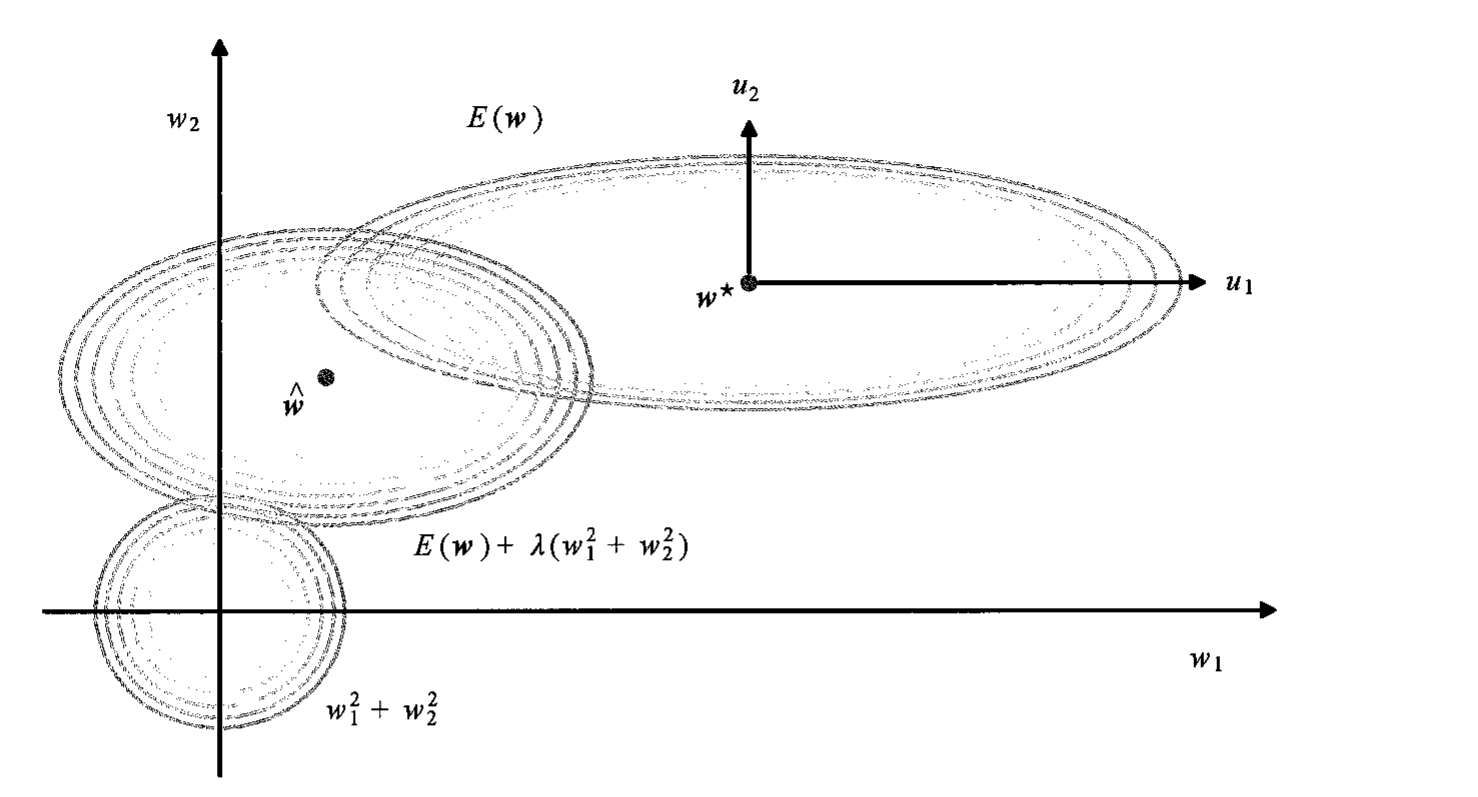
\includegraphics[width=0.78\textwidth]{ch09-fig9-3-weight-decay-contours.png}
\caption{二次误差函数与平方和正则化项 $\lambda(w_{1}^{2}+w_{2}^{2})$ 的误差函数等值线（红色）、正则化项等值线（绿色），以及两者的线性组合等值线（蓝色）。这里参数空间中的轴已经旋转以与未正则化误差函数的椭圆等值线的轴对齐。对于 $\lambda=0$，最小误差由 $\boldsymbol{w}^{*}$ 表示。当 $\lambda>0$ 时，正则化误差函数 $E(\boldsymbol{w})+\lambda(w_{1}^{2}+w_{2}^{2})$ 的最小值向原点移动。这种移动在 $w_{1}$ 方向上较大（因为未正则化误差对参数值相对不敏感），在 $w_{2}$ 方向上较小，这是误差与参数值高度相关导致的。正则化项有效地抑制了对网络预测准确性影响较小的参数}
\label{figure:ch09-权重衰减等值线}
\end{figure}

可以看到，正则化项的效果是缩小权重参数的大小。然而，正则化项对于参数 $w_{1}$ 的效果更大，因为未正则化的误差对 $w_{1}$ 值的敏感性远低于对 $w_{2}$ 值的敏感性。直观上，只有参数 $w_{2}$ 是“活跃的”，因为输出对 $w_{1}$ 相对不敏感，正则化项会将 $w_{1}$ 推向 $0$。有效参数的数量指的是正则化后仍然活跃的参数的数目，这个概念可以从 Bayes 学派或频率学派的角度形式化（Bishop，2006；Hastie，Tibshirani，and Friedman，2009）。对于 $\lambda\to\infty$，所有参数都被推向 $0$，有效参数的数量因此为 $0$。随着 $\lambda$ 的减小，有效参数的数量开始增加，直至 $\lambda=0$ 时，有效参数的数量等于模型中实际参数的总数。我们发现，通过正则化控制模型复杂性与通过限制参数数量控制模型复杂性有相似之处。

\subsection{一致性正则化项}\label{subsection:ch09-一致性正则化}

简单权重衰减形式［\eqref{align:ch09-正则化误差}］的一个缺陷是，它破坏了网络映射的某些我们想要的变换特性。为了说明这一点，考虑一个有两层权重和线性输出单元的多层感知机网络，该网络从一组输入变量 $\{x_{i}\}$ 映射到一组输出变量 $\{y_{k}\}$。第一隐藏层（简称隐层）的隐藏单元的激活由下式给出：
\begin{align}
z_{j}=h\!\left(\sum_{i}w_{ji}x_{i}+w_{j0}\right),
\label{align:ch09-隐层激活}
\end{align}
而输出单元的激活由下式给出：
\begin{align}
y_{k}=\sum_{j}w_{kj}z_{j}+w_{k0}.
\label{align:ch09-输出激活}
\end{align}
假设我们对输入数据进行如下线性变换：
\begin{align}
x_{i}\longrightarrow\tilde{x}_{i}=ax_{i}+b.
\label{align:ch09-输入线性变换}
\end{align}
然后，我们可以通过对从输入到隐藏层单元的权重和偏置进行相应的线性变换，来保证网络执行的映射不变（见\cref{exercise:ch09-04}）。下面把这一要求形式化。

\begin{definition}[线性变换一致性]\label{definition:ch09-一致性}
设 $\mathcal{G}$ 是由输入、输出变量的可逆线性（仿射）变换诱导的一族参数变换：对每个 $g\in\mathcal{G}$，用 $g(\boldsymbol{w})$ 表示使网络所表示的输入—输出映射保持不变的参数。若正则化项 $\Omega$ 满足
\begin{align*}
\Omega(g(\boldsymbol{w}))=\Omega(\boldsymbol{w}),\qquad g\in\mathcal{G},
\end{align*}
则称 $\Omega$ 与这些线性变换\textbf{一致}（consistent）；否则称 $\Omega$ 破坏了相应的变换特性。
\end{definition}

% SUPPLEMENT: parent=definition:ch09-一致性; kind=motivation; location=紧随其后的 remark（重构新增）
\begin{remark}（重构新增）\cref{definition:ch09-一致性}的要求不是“网络输出不变”，而是“正则化项在等价的参数表示上取相同的值”。这两件事必须分开：网络映射在参数变换下保持不变，是模型结构本身的性质；正则化项若不保持不变，就会在两个等价的网络之间人为地偏爱一个。由于参数化本身存在冗余（把第一层权重乘以 $a$、偏置作相应平移，可以表示同一个函数），任何只依赖参数的先验都会对这种冗余敏感。一致性正是要求正则化项对冗余“视而不见”。这也解释了为什么简单权重衰减会失败：它把权重和偏置一视同仁地惩罚，而偏置的平移与权重的缩放并不是同一回事。
\end{remark}

\begin{proposition}[网络映射的线性变换不变性]\label{proposition:ch09-网络变换不变性}
在由\eqref{align:ch09-隐层激活}与\eqref{align:ch09-输出激活}定义的两层网络中，若输入按\eqref{align:ch09-输入线性变换}变换，第一层参数按
\begin{align}
w_{ji}\longrightarrow\tilde{w}_{ji}=\frac{1}{a}w_{ji},
\label{align:ch09-第一层权重变换}
\end{align}
\begin{align}
w_{j0}\longrightarrow\tilde{w}_{j0}=w_{j0}-\frac{b}{a}\sum_{i}w_{ji}
\label{align:ch09-第一层偏置变换}
\end{align}
变换，则隐层激活 $z_{j}$ 保持不变。进一步，若输出按
\begin{align}
y_{k}\longrightarrow\tilde{y}_{k}=cy_{k}+d
\label{align:ch09-输出变换}
\end{align}
变换，第二层参数按
\begin{align}
w_{kj}\longrightarrow\tilde{w}_{kj}=cw_{kj},
\label{align:ch09-第二层权重变换}
\end{align}
\begin{align}
w_{k0}\longrightarrow\tilde{w}_{k0}=cw_{k0}+d
\label{align:ch09-第二层偏置变换}
\end{align}
变换，则新网络的输出恰为 $\tilde{y}_{k}=cy_{k}+d$。
\end{proposition}

\begin{proof}
（重构新增）对第一层，把\eqref{align:ch09-输入线性变换}至\eqref{align:ch09-第一层偏置变换}代入：
\begin{align*}
\sum_{i}\tilde{w}_{ji}\tilde{x}_{i}+\tilde{w}_{j0}
&=\sum_{i}\frac{w_{ji}}{a}(ax_{i}+b)+w_{j0}-\frac{b}{a}\sum_{i}w_{ji}\\
&=\sum_{i}w_{ji}x_{i}+\frac{b}{a}\sum_{i}w_{ji}+w_{j0}-\frac{b}{a}\sum_{i}w_{ji}\\
&=\sum_{i}w_{ji}x_{i}+w_{j0}.
\end{align*}
故 $z_{j}=h(\sum_{i}w_{ji}x_{i}+w_{j0})$ 不变。对第二层，由 $z_{j}$ 不变及\eqref{align:ch09-第二层权重变换}、\eqref{align:ch09-第二层偏置变换}，
\begin{align*}
\sum_{j}\tilde{w}_{kj}z_{j}+\tilde{w}_{k0}=\sum_{j}cw_{kj}z_{j}+cw_{k0}+d=c\Bigl(\sum_{j}w_{kj}z_{j}+w_{k0}\Bigr)+d=cy_{k}+d,
\end{align*}
这正是\eqref{align:ch09-输出变换}。
\end{proof}

% SUPPLEMENT: parent=proposition:ch09-网络变换不变性; kind=motivation; location=紧随其后的 remark（重构新增）
\begin{remark}（重构新增）\cref{proposition:ch09-网络变换不变性}中的两组变换是“同一函数的两种参数化”的显式构造：第一组把输入仿射变换吸收进第一层，第二组把输出仿射变换吸收进第二层。注意第一层权重按 $1/a$ 缩放而不是按 $a$ 缩放：输入被放大 $a$ 倍后，要得到相同的加权和，权重必须缩小 $a$ 倍。偏置的修正项 $-\frac{b}{a}\sum_{i}w_{ji}$ 则抵消输入平移 $b$ 带来的常数偏移。这些公式是\cref{proposition:ch09-一致性正则项}的直接前提；它们也说明，若对权重和偏置施加各向同性的二次惩罚，两个等价的参数化会得到不同的惩罚值，从而破坏一致性。
\end{remark}

如果使用原始数据训练一个网络，并使用输入和/或目标变量经过上述某种线性变换的数据训练另一个网络，那么一致性要求我们应该得到等价网络，它们区别仅仅在于是否对权重做了线性变换。任何正则化项都应该与这种性质一致，否则就会任意地偏好一种解而不是另一种等价的解。显然，简单权重衰减形式［\eqref{align:ch09-正则化误差}］因为平等地惩罚所有权重和偏置，所以不满足这一性质。

为此，我们需要寻找一个在线性变换［\eqref{align:ch09-第一层权重变换}、\eqref{align:ch09-第一层偏置变换}、\eqref{align:ch09-第二层权重变换}和\eqref{align:ch09-第二层偏置变换}］下不变的正则化项。这要求正则化项对权重的重新缩放和偏置的移动保持不变。这样的正则化项由下式给出：
\begin{align}
\frac{\lambda_{1}}{2}\sum_{w\in\mathcal{W}_{1}}w^{2}+\frac{\lambda_{2}}{2}\sum_{w\in\mathcal{W}_{2}}w^{2},
\label{align:ch09-一致性正则项}
\end{align}
其中 $\mathcal{W}_{1}$ 表示第一层的权重集合，$\mathcal{W}_{2}$ 表示第二层的权重集合，且偏置被排除在求和之外。原书接着指出，只要使用 $\lambda_{1}\to a^{1/2}\lambda_{1}$ 和 $\lambda_{2}\to c^{-1/2}\lambda_{2}$ 来重新缩放正则化参数，这个正则化项在权重变换下就会保持不变。

\begin{remark}（重构新增，原文问题说明）上述缩放指数按原书照译，但按\eqref{align:ch09-第一层权重变换}与\eqref{align:ch09-第二层权重变换}逐项计算，它并不能使\eqref{align:ch09-一致性正则项}保持不变：变换后第一层项为 $\frac{\lambda_{1}}{2a^{2}}\sum_{w\in\mathcal{W}_{1}}w^{2}$，要等于原来的 $\frac{\lambda_{1}}{2}\sum w^{2}$ 必须取 $\lambda_{1}'=a^{2}\lambda_{1}$；同理第二层项变为 $\frac{\lambda_{2}c^{2}}{2}\sum w^{2}$，必须取 $\lambda_{2}'=c^{-2}\lambda_{2}$。原书印作 $a^{1/2}$ 与 $c^{-1/2}$，按上述计算指数应为 $2$ 与 $-2$，应属排版或翻译中的笔误。下面\cref{proposition:ch09-一致性正则项}给出修正后的陈述与证明；正文其余部分不受影响。
\end{remark}

\begin{proposition}[一致性正则项]\label{proposition:ch09-一致性正则项}
在\cref{proposition:ch09-网络变换不变性}的记号下，正则化项\eqref{align:ch09-一致性正则项}在参数变换\eqref{align:ch09-第一层权重变换}、\eqref{align:ch09-第二层权重变换}下保持不变，当且仅当正则化系数按
\begin{align*}
\lambda_{1}\longmapsto a^{2}\lambda_{1},\qquad \lambda_{2}\longmapsto c^{-2}\lambda_{2}
\end{align*}
重新缩放。特别地，偏置不出现在\eqref{align:ch09-一致性正则项}中，因此对偏置的平移不变。
\end{proposition}

\begin{proof}
（重构新增）记变换后的系数为 $\lambda_{1}',\lambda_{2}'$。由 $\tilde{w}_{ji}=w_{ji}/a$，
\begin{align*}
\frac{\lambda_{1}'}{2}\sum_{w\in\mathcal{W}_{1}}\tilde{w}^{2}=\frac{\lambda_{1}'}{2a^{2}}\sum_{w\in\mathcal{W}_{1}}w^{2}.
\end{align*}
要使其等于 $\frac{\lambda_{1}}{2}\sum w^{2}$，必须且只需 $\lambda_{1}'=a^{2}\lambda_{1}$。同理，由 $\tilde{w}_{kj}=cw_{kj}$，
\begin{align*}
\frac{\lambda_{2}'}{2}\sum_{w\in\mathcal{W}_{2}}\tilde{w}^{2}=\frac{\lambda_{2}'c^{2}}{2}\sum_{w\in\mathcal{W}_{2}}w^{2},
\end{align*}
要使其等于 $\frac{\lambda_{2}}{2}\sum w^{2}$，必须且只需 $\lambda_{2}'=c^{-2}\lambda_{2}$。两个条件互相独立，故命题成立。偏置不在求和中，其变换\eqref{align:ch09-第一层偏置变换}、\eqref{align:ch09-第二层偏置变换}不改变\eqref{align:ch09-一致性正则项}的值。
\end{proof}

% SUPPLEMENT: parent=proposition:ch09-一致性正则项; kind=motivation; location=紧随其后的 remark（重构新增）
\begin{remark}（重构新增）\cref{proposition:ch09-一致性正则项}给出了“按层分组、只惩罚权重、不惩罚偏置”这一做法的理由：只有这样才能与输入、输出的仿射重参数化相容。但一致性是有代价的：由于偏置完全不受惩罚，\eqref{align:ch09-一致性先验}所对应的先验是反常的（不可归一化），因为偏置可以在 $\mathbb{R}$ 上任意取值而不影响惩罚。实际使用中通常再给偏置单独加一个较弱的先验（从而主动打破平移不变性），其超参数与权重的超参数分开。这也说明“一致性”不是越彻底越好：它是一个建模选择，需要与任务真正具有的对称性相匹配。
\end{remark}

正则化项［\eqref{align:ch09-一致性正则项}］对应于参数的先验分布形式：
\begin{align}
p(\boldsymbol{w}\mid\alpha_{1},\alpha_{2})\propto\exp\!\left(-\frac{\alpha_{1}}{2}\sum_{w\in\mathcal{W}_{1}}w^{2}-\frac{\alpha_{2}}{2}\sum_{w\in\mathcal{W}_{2}}w^{2}\right).
\label{align:ch09-一致性先验}
\end{align}
注意，这种形式的先验是反常的（它们不能被规范化），因为偏置参数是不受约束的。使用反常的先验可能会对选择正则化系数，以及在 Bayes 框架内进行模型比较造成困难。因此，我们通常会为偏置设置单独的先验（从而打破平移不变性），这些先验都有自己的超参数。

我们可以通过从先验中抽取样本并绘制相应的网络函数来展示这 $4$ 个超参数的效果，如\cref{figure:ch09-先验样本}所示。先验由 $4$ 个超参数控制：$\alpha_{1}^{b}$、$\alpha_{1}^{w}$、$\alpha_{2}^{b}$ 和 $\alpha_{2}^{w}$，它们分别代表第一层偏置、第一层权重、第二层偏置和第二层权重所服从的 Gauss 分布的精度。可以看到，超参数 $\alpha_{2}^{w}$ 控制函数的竖直尺度（注意\cref{figure:ch09-先验样本}(a) 和\cref{figure:ch09-先验样本}(b) 的竖直轴具有不同的取值范围），$\alpha_{1}^{w}$ 控制函数值变化的水平尺度，$\alpha_{1}^{b}$ 控制函数值变化的水平范围。超参数 $\alpha_{2}^{b}$ 的效果此处未展示，其控制函数的竖直偏移范围。

\begin{figure}[htbp]
\centering
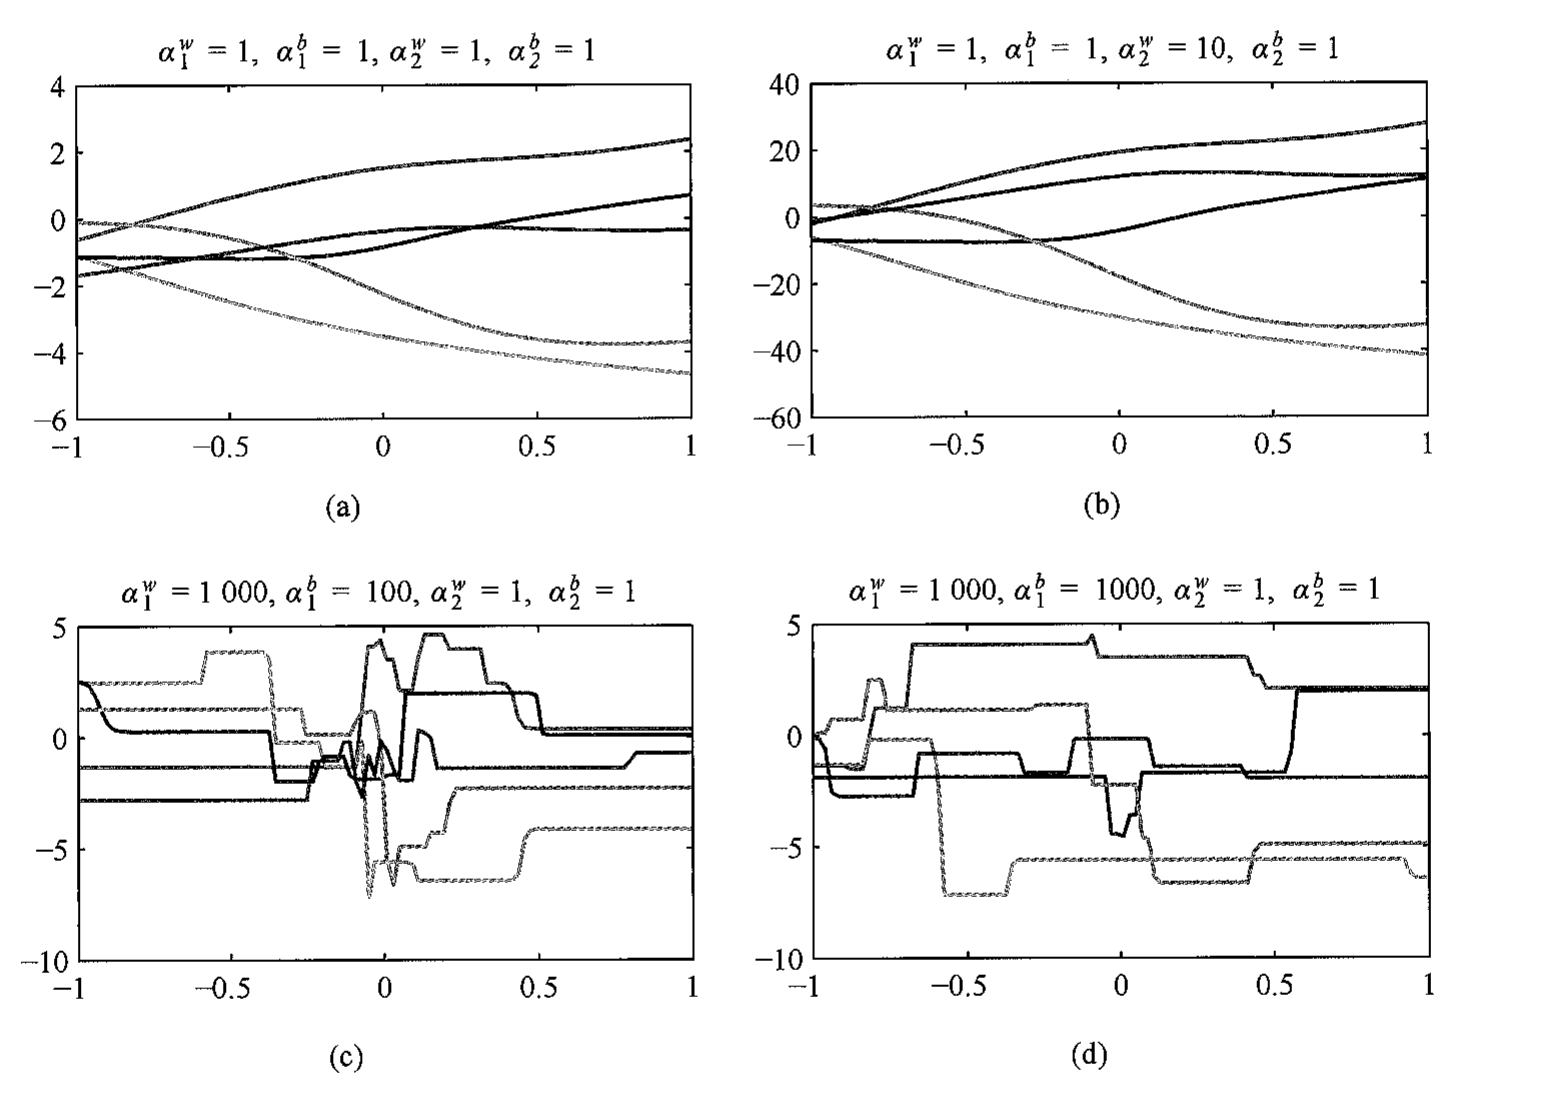
\includegraphics[width=0.86\textwidth]{ch09-fig9-4-prior-samples.png}
\caption{在具有单一输入、单一线性输出和 12 个由 tanh 函数激活的隐藏单元的双层神经网络中，旨在控制权重和偏置先验分布的超参数的效果示意图}
\label{figure:ch09-先验样本}
\end{figure}

\subsection{广义权重衰减}\label{subsection:ch09-广义权重衰减}

更一般地，考虑将权重分成任意多组 $\mathcal{W}_{k}$ 的正则化项，使得
\begin{align}
\Omega(\boldsymbol{w})=\frac{1}{2}\sum_{k}\alpha_{k}\|\boldsymbol{w}\|_{k}^{2},
\label{align:ch09-分组正则项}
\end{align}
其中
\begin{align}
\|\boldsymbol{w}\|_{k}^{2}=\sum_{j\in\mathcal{W}_{k}}w_{j}^{2}.
\label{align:ch09-分组范数}
\end{align}
例如，我们可以为多层网络中的每一层使用不同的正则化项。

\begin{definition}[分组权重衰减]\label{definition:ch09-分组权重衰减}
设参数被划分为若干互不相交的组 $\mathcal{W}_{k}$，$\boldsymbol{w}_{k}$ 表示第 $k$ 组的权重子向量。称由\eqref{align:ch09-分组正则项}与\eqref{align:ch09-分组范数}定义的 $\Omega(\boldsymbol{w})$ 为\textbf{分组权重衰减}（grouped weight decay），$\alpha_{k}>0$ 为第 $k$ 组的正则化系数（等价地，第 $k$ 组先验的精度）。
\end{definition}

% SUPPLEMENT: parent=definition:ch09-分组权重衰减; kind=motivation; location=紧随其后的 remark（重构新增）
\begin{remark}（重构新增）\cref{definition:ch09-分组权重衰减}把“一个全局 $\lambda$”推广为“每组一个 $\alpha_{k}$”，其必要性来自不同层权重的尺度差异：输入层权重的量级、隐藏层权重的量级和输出层权重的量级往往相差很大，用同一个 $\lambda$ 会使某些层被过度收缩而另一些层几乎不受约束。分组也带来新的选择问题：组划分本身是一种结构先验，划得过细等价于给每组单独调参，划得过粗又退化为全局权重衰减。\eqref{align:ch09-一致性正则项}就是按“层”分组的特例，它同时满足线性变换一致性；一般的分组则未必具有这种不变性。
\end{remark}

我们有时使用简单的二次正则化项的一般形式：
\begin{align}
\Omega(\boldsymbol{w})=\frac{\lambda}{2}\sum_{j=1}^{M}|w_{j}|^{q}.
\label{align:ch09-q范数正则}
\end{align}

\begin{definition}[$q$-范数正则化与 lasso]\label{definition:ch09-lasso}
对 $q>0$，称\eqref{align:ch09-q范数正则}为 \textbf{$q$-范数正则化项}（$q$-norm regularizer）。当 $q=1$ 时，它在统计学领域称为 \textbf{lasso}（least absolute shrinkage and selection operator）（Tibshirani，1996）；当 $q=2$ 时，它退化为\eqref{align:ch09-正则化误差}中的二次正则化项。
\end{definition}

% SUPPLEMENT: parent=definition:ch09-lasso; kind=motivation; location=紧随其后的 remark（重构新增）
\begin{remark}（重构新增）\cref{definition:ch09-lasso}中的 $q$ 控制等值线的几何形状，从而控制解的稀疏性：$q=2$ 的等值线是光滑的球面，$q=1$ 的是有尖角的菱形，$0<q<1$ 的是向坐标轴凹陷的星形。稀疏性来自“尖角”与误差椭圆相切的位置：切点落在坐标轴上，就使相应分量为零。$q<1$ 时目标函数非凸，存在多个局部极小，优化更困难；$q=1$ 是仍保持凸性的最小指数，因此成为变量选择的标准选择。注意 $q$-范数记法在 $q\neq2$ 时并不是真正的范数（不满足三角不等式），只是对 $\sum|w_{j}|^{q}$ 的简称。
\end{remark}

其中 $q=2$ 对应于\eqref{align:ch09-正则化误差}中的二次正则化项。\cref{figure:ch09-q等值线}显示了不同 $q$ 值的正则化函数的等值线。

\begin{figure}[htbp]
\centering
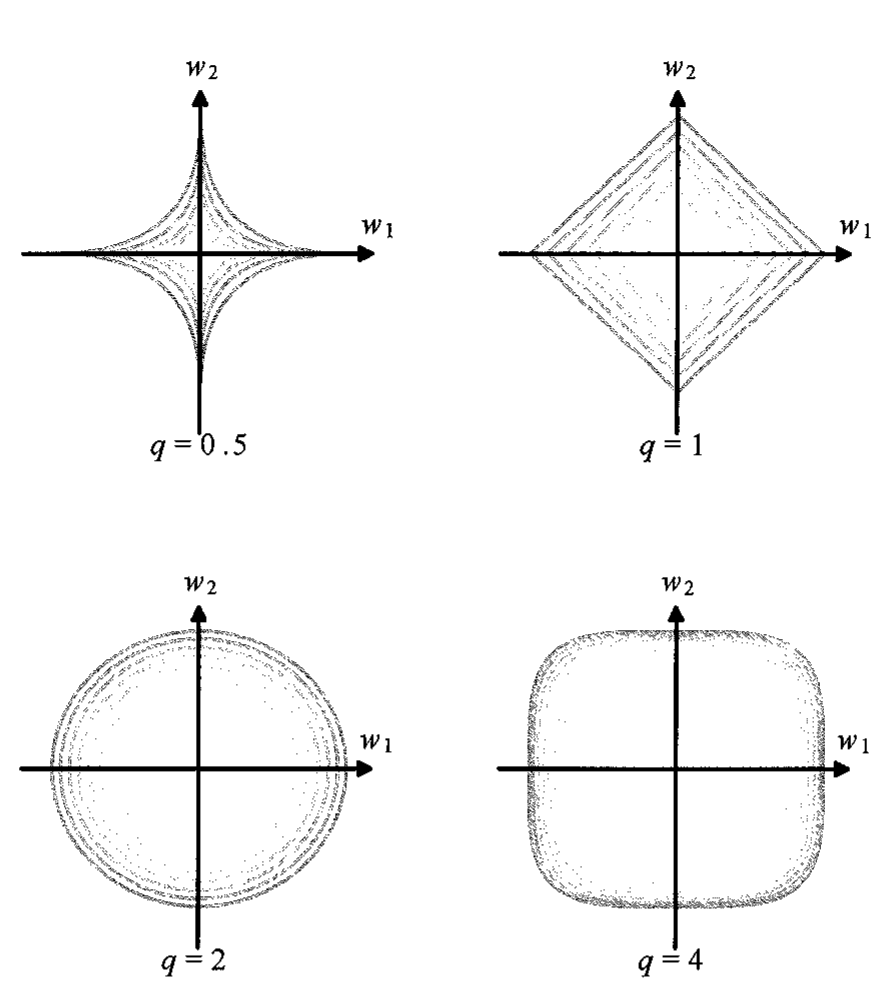
\includegraphics[width=0.55\textwidth]{ch09-fig9-5-q-contours.png}
\caption{不同 $q$ 值的正则化函数的等值线}
\label{figure:ch09-q等值线}
\end{figure}

当 $q=1$ 时，形如\eqref{align:ch09-q范数正则}的正则化项在统计学领域称为 lasso（Tibshirani，1996）。对于二次误差函数，它的性质是，如果 $\lambda$ 足够大，系数 $w_{j}$ 将趋于零，从而得到一个稀疏的模型，对应的基函数不起作用。为了说明这一点，考虑最小化下式给出的正则化误差函数：
\begin{align}
E(\boldsymbol{w})+\frac{\lambda}{2}\sum_{j=1}^{M}|w_{j}|^{q}.
\label{align:ch09-lasso目标}
\end{align}
这等价于在约束条件（见\cref{exercise:ch09-05}）
\begin{align}
\sum_{j=1}^{M}|w_{j}|^{q}\leqslant\eta
\label{align:ch09-lasso约束}
\end{align}
下最小化未正则化的误差函数 $E(\boldsymbol{w})$，其中 $\eta$ 有一个合适的取值。这两种方法可以通过 Lagrange 乘子法关联起来（参见\hyperref[chapter:appC-Lagrange乘子]{附录\ref*{chapter:appC-Lagrange乘子}}）。

\begin{proposition}[lasso 的约束等价形式]\label{proposition:ch09-lasso约束等价}
设 $E:\mathbb{R}^{M}\to\mathbb{R}$ 为凸函数，$q\geqslant1$，并设约束问题
\begin{align*}
\min_{\boldsymbol{w}}E(\boldsymbol{w})\quad\text{使得}\quad\sum_{j=1}^{M}|w_{j}|^{q}\leqslant\eta
\end{align*}
满足 Slater 条件（存在严格可行点）。则对每个 $\lambda>0$，存在 $\eta=\eta(\lambda)\geqslant0$，使得\eqref{align:ch09-lasso目标}的任一最小点都是该约束问题的最小点；反之，对每个 $\eta>0$，存在 $\lambda=\lambda(\eta)\geqslant0$，使得约束问题的任一最小点都是\eqref{align:ch09-lasso目标}的最小点。
\end{proposition}

\begin{proof}
（重构新增）记 $g(\boldsymbol{w})=\sum_{j}|w_{j}|^{q}$。\eqref{align:ch09-lasso目标}是 $\min_{\boldsymbol{w}}E(\boldsymbol{w})+\frac{\lambda}{2}g(\boldsymbol{w})$，其 Lagrange 函数可写为
\begin{align*}
\mathcal{L}(\boldsymbol{w},\mu)=E(\boldsymbol{w})+\frac{\mu}{2}\bigl(g(\boldsymbol{w})-\eta\bigr),\qquad \mu\geqslant0.
\end{align*}
由凸性及 Slater 条件，KKT 条件是最优性的充要条件：存在 $\mu\geqslant0$ 使
\begin{align*}
\boldsymbol{0}\in\partial E(\boldsymbol{w})+\frac{\mu}{2}\partial g(\boldsymbol{w}),\qquad \mu\bigl(g(\boldsymbol{w})-\eta\bigr)=0.
\end{align*}
取 $\lambda=\mu$ 即知约束问题的 KKT 点满足\eqref{align:ch09-lasso目标}的一阶最优性条件；凸情形下这也是充分条件，故约束问题的最小点是\eqref{align:ch09-lasso目标}的最小点。反过来，给定 $\lambda>0$，令 $\boldsymbol{w}_{\lambda}$ 为\eqref{align:ch09-lasso目标}的最小点，取 $\eta=g(\boldsymbol{w}_{\lambda})$，则 $\boldsymbol{w}_{\lambda}$ 满足约束且 KKT 条件中的互补松弛成立，从而是约束问题的最小点。$\eta$ 与 $\lambda$ 的对应由 $g(\boldsymbol{w}_{\lambda})$ 关于 $\lambda$ 的单调性给出：$\lambda$ 增大时最优解的 $g$ 值不增，故 $\eta(\lambda)$ 单调不增；在 $g$ 严格凸且解唯一的区域可逆。
\end{proof}

% SUPPLEMENT: parent=proposition:ch09-lasso约束等价; kind=motivation; location=紧随其后的 remark（重构新增）
\begin{remark}（重构新增）\cref{proposition:ch09-lasso约束等价}把“惩罚形式”和“约束形式”视为同一个问题的两种参数化，这在几何上解释了\cref{figure:ch09-lasso稀疏}：约束形式把解限制在半径为 $\eta$ 的 $q$-球内，惩罚形式则用等值线去“推”解。两者只在凸情形下等价；若 $E$ 非凸或 $q<1$，KKT 只是必要条件，可能出现局部解与全局解不一致。还要注意 $\eta$ 与 $\lambda$ 的对应依赖数据（通过 $E$ 的曲率），并不是一个固定的换算公式；\cref{exercise:ch09-05}要求讨论这一关系。
\end{remark}

模型稀疏的原因可以通过\cref{figure:ch09-lasso稀疏}说明：该图显示了误差函数在约束条件\eqref{align:ch09-lasso约束}下的最小值。随着 $\lambda$ 增大，更多参数将趋于零。相比之下，二次正则化项不会要求权重参数为零，只会将 $w_{j}$ 减小到一个较小值。lasso 正则化项提供了一个稀疏解，其中 $w_{j}=0$。

\begin{figure}[htbp]
\centering
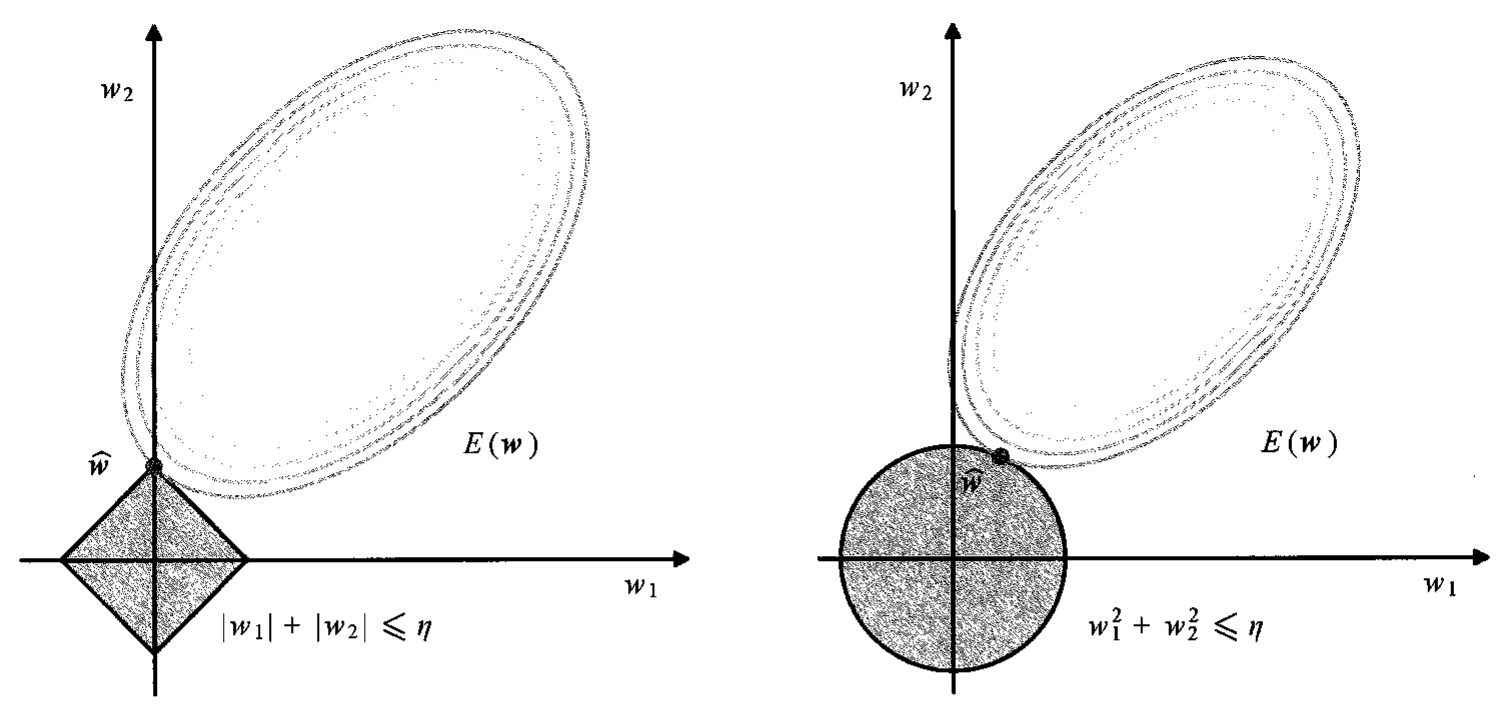
\includegraphics[width=0.88\textwidth]{ch09-fig9-6-lasso-contours.png}
\caption{未正则化的误差函数的等值线（红色）以及两种情况的约束条件［\eqref{align:ch09-lasso约束}］的示意图。左侧是 $q=1$ 时的 lasso 正则化项，右侧是 $q=2$ 时的二次正则化项。其中参数向量 $\boldsymbol{w}$ 的最优值由 $\hat{\boldsymbol{w}}$ 表示。lasso 正则化项提供了一个稀疏解，其中 $\hat{w}_{1}=0$，而二次正则化项仅将 $w_{1}$ 减至一个较小的值}
\label{figure:ch09-lasso稀疏}
\end{figure}

正则化使得我们在有限大小的数据集上训练复杂模型的同时不会造成严重的过拟合，这本质上是通过限制有效模型的复杂度来实现的。这就让确定最优的模型复杂度问题从寻找适当数量的可学习参数变为确定合适的正则化系数 $\lambda$。我们将在下一节讨论模型复杂度问题。

\end{document}
